\documentclass[tikz,border=3pt,12pt]{standalone}
\usepackage[T1]{fontenc}
\usepackage{lmodern,amsmath,amssymb}
\usetikzlibrary{arrows.meta,calc,positioning,fit}
\begin{document}
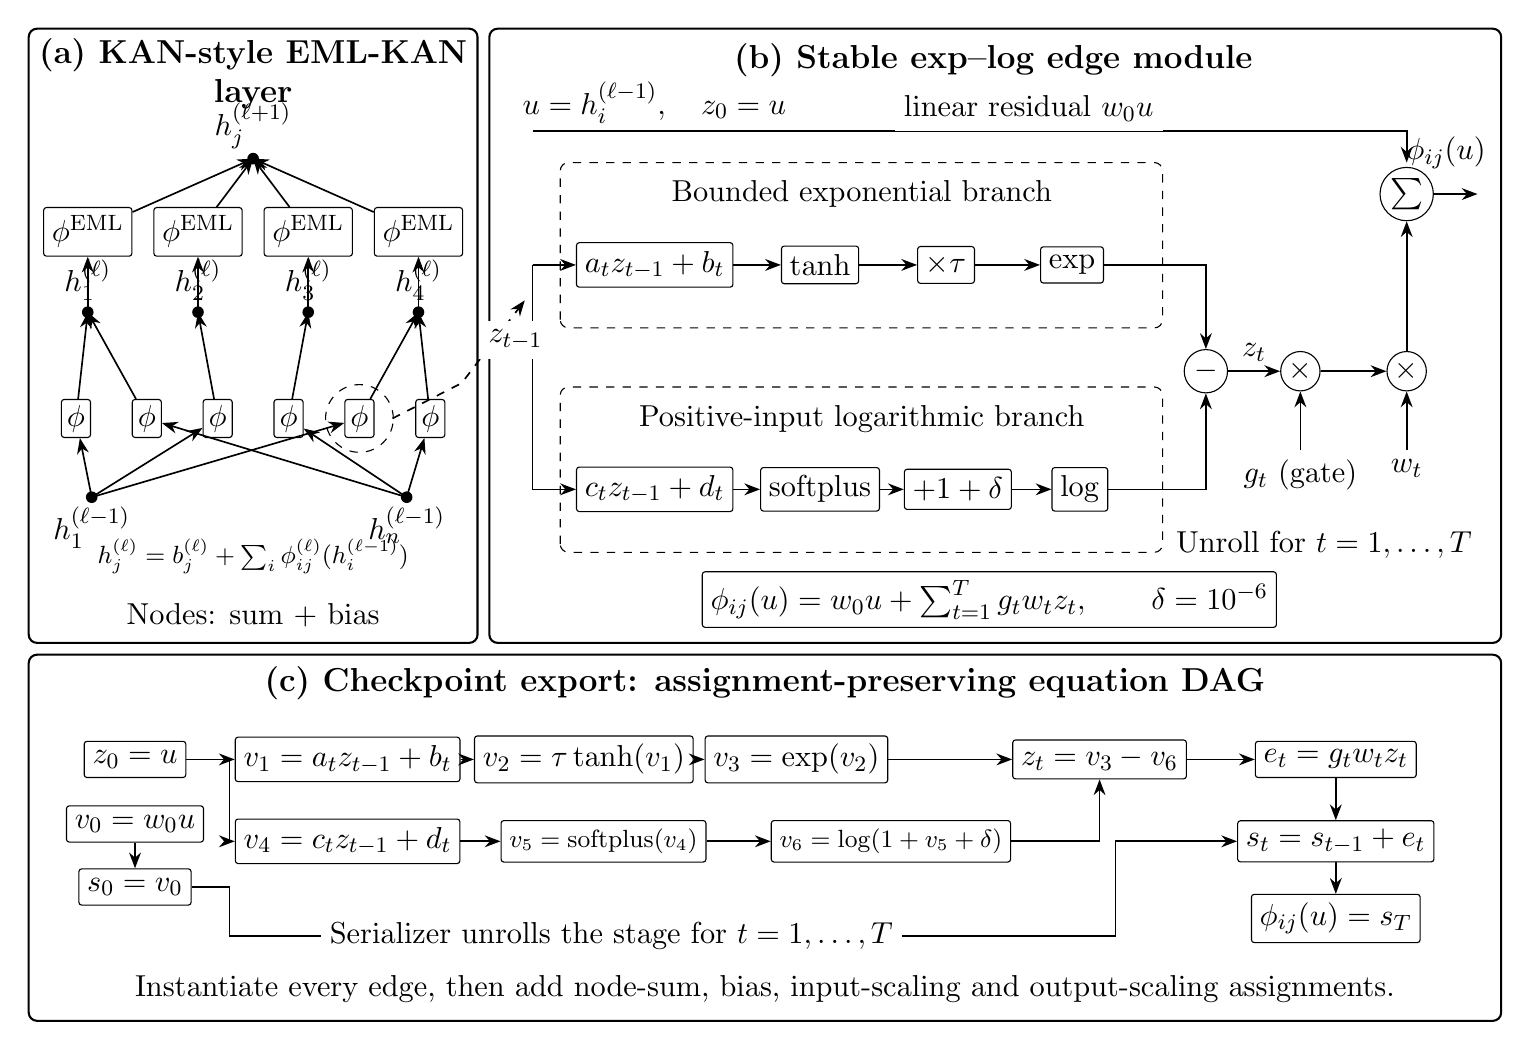
\begin{tikzpicture}[x=1cm,y=1cm,>=Stealth,
 font=\fontsize{11.3}{12.4}\selectfont,
 box/.style={draw,rounded corners=1pt,fill=white,inner sep=3pt,minimum height=.46cm},
 arrow/.style={->,line width=.6pt},
 panel/.style={draw,rounded corners=3pt,line width=.75pt},
 title/.style={font=\bfseries\fontsize{12.7}{14}\selectfont}]
\draw[panel] (0,4.8) rectangle (5.7,12.6);
\draw[panel] (5.85,4.8) rectangle (18.7,12.6);
\draw[panel] (0,0) rectangle (18.7,4.65);
\node[title,align=center] at (2.85,12.03) {(a) KAN-style EML-KAN\\layer};
\node[title] at (12.25,12.2) {(b) Stable exp--log edge module};
\node[title] at (9.35,4.29) {(c) Checkpoint export: assignment-preserving equation DAG};

% Layer aggregation, with one edge selected for the enlarged module.
\coordinate (u1) at (.8,6.65);\coordinate (u2) at (4.8,6.65);
\coordinate (h1) at (.75,9.0);\coordinate (h2) at (2.15,9.0);
\coordinate (h3) at (3.55,9.0);\coordinate (h4) at (4.95,9.0);
\coordinate (out) at (2.85,10.95);
\foreach \v in {u1,u2,h1,h2,h3,h4,out}{\fill (\v) circle (2.1pt);}
\node[above] at (out) {$h_j^{(\ell+1)}$};
\foreach \k/\x in {1/.75,2/2.15,3/3.55,4/4.95}{
 \node[above] at (\x,9.02) {$h_{\k}^{(\ell)}$};
 \node[box] (e\k) at (\x,10.02) {$\phi^{\mathrm{EML}}$};
 \draw[arrow] (h\k)--(e\k);\draw[arrow] (e\k)--(out);
}
\foreach \k/\x in {1/.6,2/1.5,3/2.4,4/3.3,5/4.2,6/5.1}{
 \node[box,inner sep=2pt] (l\k) at (\x,7.65) {$\phi$};
}
\draw[arrow] (u1)--(l1);\draw[arrow] (u1)--(l3);\draw[arrow] (u1)--(l5);
\draw[arrow] (u2)--(l2);\draw[arrow] (u2)--(l4);\draw[arrow] (u2)--(l6);
\draw[arrow] (l1)--(h1);\draw[arrow] (l2)--(h1);
\draw[arrow] (l3)--(h2);\draw[arrow] (l4)--(h3);
\draw[arrow] (l5)--(h4);\draw[arrow] (l6)--(h4);
\node[below] at (u1) {$h_1^{(\ell-1)}$};\node[below] at (u2) {$h_n^{(\ell-1)}$};
\draw[dashed] (l5) circle (.43cm);
\draw[arrow,dashed] (4.62,7.65)--(5.5,8.1)--(6.3,9.15);
\node[font=\small] at (2.85,5.9) {$h_j^{(\ell)}=b_j^{(\ell)}+\sum_i\phi_{ij}^{(\ell)}(h_i^{(\ell-1)})$};
\node[align=center,font=\fontsize{10.7}{12}\selectfont] at (2.85,5.15) {Nodes: sum + bias};

% Enlarged edge module, retaining branch order and residual aggregation.
\node[anchor=west] at (6.15,11.66) {$u=h_i^{(\ell-1)},\quad z_0=u$};
\draw[arrow] (6.4,11.3)--(17.5,11.3)--(17.5,10.9);
\node[above,fill=white] at (12.7,11.3) {linear residual $w_0u$};
\node[draw,circle,inner sep=1pt,minimum size=.65cm] (sum) at (17.5,10.5) {$\sum$};
\draw[arrow] (sum)--(18.4,10.5);
\node[above,align=center] at (18,10.7) {$\phi_{ij}(u)$};
\draw[dashed,rounded corners=3pt] (6.75,8.8) rectangle (14.4,10.9);
\node[align=center] at (10.58,10.5) {Bounded exponential branch};
\node[box] (a) at (7.95,9.6) {$a_tz_{t-1}+b_t$};
\node[box] (tanh) at (10.05,9.6) {$\tanh$};
\node[box] (scale) at (11.65,9.6) {$\times\tau$};
\node[box] (exp) at (13.25,9.6) {$\exp$};
\draw[arrow] (a)--(tanh);\draw[arrow] (tanh)--(scale);\draw[arrow] (scale)--(exp);
\draw[dashed,rounded corners=3pt] (6.75,5.95) rectangle (14.4,8.05);
\node[align=center] at (10.58,7.65) {Positive-input logarithmic branch};
\node[box] (c) at (7.95,6.75) {$c_tz_{t-1}+d_t$};
\node[box] (softplus) at (10.05,6.75) {$\operatorname{softplus}$};
\node[box] (add) at (11.8,6.75) {$+1+\delta$};
\node[box] (log) at (13.35,6.75) {$\log$};
\draw[arrow] (c)--(softplus);\draw[arrow] (softplus)--(add);\draw[arrow] (add)--(log);
\draw[arrow] (6.4,9.6)--(a);\draw[arrow] (6.4,9.6)--(6.4,6.75)--(c);
\node[anchor=east,fill=white] at (6.65,8.65) {$z_{t-1}$};
\node[draw,circle,inner sep=1pt,minimum size=.55cm] (minus) at (14.95,8.25) {$-$};
\draw[arrow] (exp)--(14.95,9.6)--(minus);
\draw[arrow] (log)--(14.95,6.75)--(minus);
\node[draw,circle,inner sep=1pt,minimum size=.5cm] (gate) at (16.15,8.25) {$\times$};
\node[draw,circle,inner sep=1pt,minimum size=.5cm] (coef) at (17.5,8.25) {$\times$};
\draw[arrow] (minus)--node[above]{$z_t$}(gate);\draw[arrow] (gate)--(coef);
\draw[arrow] (16.15,7.25)--(gate);\node[below] at (16.15,7.25) {$g_t$ (gate)};
\draw[arrow] (17.5,7.25)--(coef);\node[below] at (17.5,7.25) {$w_t$};
\draw[arrow] (coef)--(sum);
\node[box] at (12.2,5.35) {$\phi_{ij}(u)=w_0u+\sum_{t=1}^{T}g_tw_tz_t,\qquad\delta=10^{-6}$};
\node[font=\fontsize{10.7}{12}\selectfont] at (16.45,6.05) {Unroll for $t=1,\ldots,T$};

% One recurrence stage: ordered scalar assignments and explicit shared nodes.
\node[box] (init) at (1.35,3.32) {$z_0=u$};
\node[box] (vzero) at (1.35,2.5) {$v_0=w_0u$};
\node[box] (szero) at (1.35,1.7) {$s_0=v_0$};
\draw[arrow] (vzero)--(szero);
\node[box] (vone) at (4.05,3.32) {$v_1=a_tz_{t-1}+b_t$};
\node[box] (vtwo) at (7.05,3.32) {$v_2=\tau\tanh(v_1)$};
\node[box] (vthree) at (9.75,3.32) {$v_3=\exp(v_2)$};
\node[box] (vfour) at (4.05,2.28) {$v_4=c_tz_{t-1}+d_t$};
\node[box,font=\small] (vfive) at (7.3,2.28) {$v_5=\operatorname{softplus}(v_4)$};
\node[box,font=\small] (vsix) at (10.95,2.28) {$v_6=\log(1+v_5+\delta)$};
\draw[arrow] (init)--(vone);\draw[arrow] (2.55,3.32)--(2.55,2.28)--(vfour);
\draw[arrow] (vone)--(vtwo);\draw[arrow] (vtwo)--(vthree);
\draw[arrow] (vfour)--(vfive);\draw[arrow] (vfive)--(vsix);
\node[box] (zt) at (13.6,3.32) {$z_t=v_3-v_6$};
\draw[arrow] (vthree)--(zt);\draw[arrow] (vsix)-|(zt);
\node[box] (et) at (16.6,3.32) {$e_t=g_tw_tz_t$};\draw[arrow] (zt)--(et);
\node[box] (st) at (16.6,2.28) {$s_t=s_{t-1}+e_t$};\draw[arrow] (et)--(st);
\node[box] (phi) at (16.6,1.3) {$\phi_{ij}(u)=s_T$};\draw[arrow] (st)--(phi);
\draw[arrow] (szero)--(2.55,1.7)--(2.55,1.08)--(13.8,1.08)--(13.8,2.28)--(st);
\node[fill=white,font=\fontsize{10.7}{12}\selectfont] at (7.4,1.08) {Serializer unrolls the stage for $t=1,\ldots,T$};
\node[align=center,font=\fontsize{11.1}{12.4}\selectfont] at (9.35,.4) {Instantiate every edge, then add node-sum, bias, input-scaling and output-scaling assignments.};
\end{tikzpicture}
\end{document}
